\documentclass[pdf, aspectratio=169, 12pt]{beamer}
\usepackage[]{hyperref, graphicx, siunitx, lmodern, tikz, booktabs, physics, multicol}
\usepackage[mode=buildnew]{standalone}
\usepackage{pdfpc-commands}
\usepackage{pgfplots}
\pgfplotsset{compat=1.16}

\usetheme[sols]{Python}

\graphicspath{ {Images/} }

\sisetup{per-mode=symbol}
\usetikzlibrary{calc, patterns, decorations.markings, decorations.pathmorphing, shapes, fit}

%Preamble
\title{Making the Most of Arcade}
\author{Jed Rembold}
\date{April 17, 2020}

\begin{document}

\begin{frame}{Announcements}
	\begin{itemize}
		\item Homework
			\begin{itemize}
				\item Homework 10 due tonight! Last HW! Celebrate! :)
				\item You are going to start getting a bunch of graded things back this weekend. I'm almost through my backlog in my other classes. \alert{Soooo} sorry for the delay. :(
			\end{itemize}
		\item Projects
			\begin{itemize}
				\item Should have gotten an email (and it is posted on Campuswire) for a poll about the final project
				\item We'll talk more about them today in class
			\end{itemize}
		\item Polling: \nolinkurl{rembold-class.ddns.net}
	\end{itemize}
\end{frame}

\begin{frame}[fragile]{Review Question}
	\begin{columns}
		\column{0.5\textwidth}

		\vspace{3mm}
		\small
		Suppose I ran the class to the right, created an instance of it, and then pressed the followed keys: w, w,  a, s, w. Which location below would show where the circle was at the end?
		\begin{center}
			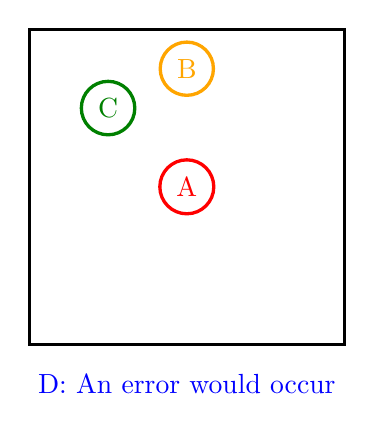
\begin{tikzpicture}
				\draw[very thick] (-2,-2) rectangle (2,2);
				\node[circle, draw, very thick, Red] at (0,0) {A};
				\node[circle, draw, very thick, Orange] at (0,1.5) {B};
				\node[circle, draw, very thick, Green] at (-1,1) {C};
				\node[Blue] at (0,-2.5) {D: An error would occur};
			\end{tikzpicture}
			
		\end{center}
		\exsol{D}
		\column{0.5\textwidth}
		\scriptsize
		\begin{pythoncode}
			import arcade

			class A(arcade.Window):
				def __init_(self):
					arcade.Window.__init__(100,100,'')
					self.x = 50
					self.y = 50
					self.r = 10

				def on_draw(self):
					arcade.start_render()
					arcade.draw_circle_filled(
									self.x,
									self.y,
									self.r,
									arcade.color.RED)

				def on_key_press(key, modifier):
					if key == arcade.key.W:
						self.y += 10
					elif key == arcade.key.A
						self.x -= 10
		\end{pythoncode}
	\end{columns}
\end{frame}

\begin{frame}{Projects}
	\vspace{5mm}
	\begin{itemize}
		\item Mostly groups of 2 or 3, which I will be creating and sending out
			\begin{itemize}
				\item Care about your group members, let me know in the poll!
			\end{itemize}
		\item Projects are pretty much open to whatever you want or are interested in! I am happy to help with ideas if you like.
		\item Will do a 10 min + question presentation/video on the project on our last day of classes
			\begin{itemize}
				\item Can do live or prerecord if timezones make things difficult
				\item Should include:
					\begin{itemize}
						\item What your project was
						\item How you approached it and divided up the problem
						\item Who worked on what parts
						\item How it came together and works
						\item A demo or screencapture of it working would be nice!
					\end{itemize}
			\end{itemize}
		\item Code will be submitted to Github, but besides the presentation and code no other ``output'' is necessary.
	\end{itemize}
\end{frame}

\begin{frame}{Timeline}
	\begin{itemize}
		\item Campuswire and Github groups will be made for each grouping
		\item Monday's class will focus on planning a project and collaborative coding
		\item No class on Wednesday due to SSRD
		\item Friday we play Digital Dodgeball
		\item All classes and labs the following week are just set aside for working on the projects, meeting with your group members, or asking me questions
	\end{itemize}
\end{frame}

\begin{frame}{Refactoring Arcade Code for Flexibility}
	\begin{itemize}
		\item When things start getting too complicated in one function or class, it may be time to break some of that logic out to another class/function!
		\item A good candidate can be breaking an ``object'' you are drawing to the screen out into its own class.
			\begin{itemize}
				\item Will still probably need to provide drawing and update methods for that class.
			\end{itemize}
	\end{itemize}
\end{frame}

\begin{frame}{Working with Sprites}
	\begin{itemize}
		\item We've played around a bit before with adding Sprites (images) to the screen
		\item By adding them to a \pyi{arcade.SpriteList} we get an efficient and easy way to:
			\begin{itemize}
				\item Draw everything on the list to the screen
				\item Update the positions of everything in the list
				\item Check such things as collisions between objects in different lists
				\item Set up basic physics between different types of objects
			\end{itemize}
	\end{itemize}
\end{frame}

\begin{frame}{Ah yeah Physics}
	\begin{itemize}
		\item You can always set up your own movement systems
		\item Platformers tend to be a bit more tricky since you have to check for collisions with the terrain to know when to stand on something
		\item Arcade has a simple physics engine you can use for this
			\begin{itemize}
				\item You give it the things you can the physics to act on,
				\item The solid land or terrain you want to be impassable,
				\item and a strength of gravity
			\end{itemize}
		\item Don't forget to update the physics engine then in \pyi{on_update}!
			
	\end{itemize}
	
\end{frame}












\end{document}

